\documentclass{report}
\usepackage[utf8]{inputenc}
\usepackage{mathtools}
\usepackage{scrextend}
\usepackage[inline]{enumitem}
\usepackage[T2A]{fontenc}
\usepackage[russiun]{babel}
\usepackage[usenames]{color}
\usepackage{colortbl}
\usepackage{float}
\usepackage{wrapfig}
\usepackage{graphicx}
\usepackage{sidecap}
\usepackage{subcaption}
\usepackage{cite}
\begin{document}

\begin{titlepage}
    \newpage
    \begin{center}
    {\bfseries Федеральное государственное автономное образовательное учреждение высшего образования  \\
    \vspace{0,5cm}
    «НАЦИОНАЛЬНЫЙ ИССЛЕДОВАТЕЛЬСКИЙ УНИВЕРСИТЕТ
    «ВЫСШАЯ ШКОЛА ЭКОНОМИКИ»
     
     \vspace{0,5cm}
     Факультет компьютерных наук
    }
    \vspace{3cm}

    
    \Large Работа\linebreak
    Introduction to LaTeX \linebreak
    \end{center}

    \vspace{5em}

   
     \hspace{70mm} 
                     Выполнил:
   
    \begin{flushright}
    Студент группы БПМИ2111 Климчук Антонина Игоревна
    \end{flushright}

    \hspace{70mm} 
    Руководитель: 
    \begin{flushright}
    Рудаков Кирилл Александрович, Приглашенный преподаватель , М департамент больших данных и информационного поиска

    \end{flushright}
     \vspace{5cm}

    \begin{center}
    Июль 2022
    \end{center}

\end{titlepage}
    
 




\begin{figure}
    \centering
    \begin{subfigure}[b]{0.3\textwidth}
        
\includegraphics[width=\textwidth]{patric.jpg}
        \caption{Патрик}
        \label{fig:gull}
    \end{subfigure}
    ~ %add desired spacing between images, e. g. ~, \quad, \qquad, \hfill etc. 
      %(or a blank line to force the subfigure onto a new line)
    \begin{subfigure}[b]{0.3\textwidth}
        
\includegraphics[width=\textwidth]{spanch_bob.jpeg}
        \caption{Спанч Боб}
        \label{fig:tiger}
    \end{subfigure}
    ~ %add desired spacing between images, e. g. ~, \quad, \qquad, \hfill etc. 
    %(or a blank line to force the subfigure onto a new line)
    \begin{subfigure}[b]{0.3\textwidth}
        
\includegraphics[width=\textwidth]{squidward.jpeg}
        \caption{Сквидвард}
        \label{fig:mouse}
    \end{subfigure}
    \caption{Картиночки}\label{fig:animals}
\end{figure}

\begin{abstract}
    Пример непрактического вопроса:” Почему люди не летают?”. Многие часто задаются этим вопросом, но не могут найти на него ответ. Однако, кто-то все-таки обдумывает эту сложную философскую проблему, возможно, именно поэтому в мире появляются комиксы с людьми,которые способны летать. Это своеобразное решение показывает нам что все-таки есть люди,которым действительно важен ответ на этот сложный, возможно, безответный вопрос.аботами.
\end{abstract}

\tableofcontents
\part{First}
\chapter{Тексты}
\section{Проблемы науки в раннее Новое время}


Научная революция послужила основным фактором для того, чтобы теологические учения отошли на задний план. Наука развивалась благодаря массовой печати книг, в которых были написаны работы в сферах астрономии, математики, физики, архитектуры, живописи, медицине (химии и биологии) - не религиозный характер. Общество нуждалось в переменах и отказе от средневековых предрассудков (в данном случае в научной сфере). Очень важным критерием этой революции стало противостояние церкви и науки.

Научная революция стала переломом в сознании человечества, в первую очередь в точных науках (астрономия, математика). Родоначальник экспериментальной науки Николай Коперник – польский ученый, он построил импровизированную обсерваторию и доказал то, что не солнце движется вокруг земли, а наоборот – земля вокруг солнца. Джордано Бруно – итальянский монах – был распространителем гелиоцентрической теории Коперника, из-за чего в 1600 году он был сожжен на костре (все опять же из-за религии). Множество технологических открытий, например, телескоп, с помощью которого была подтверждена теория Коперника, и термометр (их изобрел Галилео Галилей). 

\begin{SCfigure}[1][!h]
  \centering
  \caption{Ньютон и яблоко }
  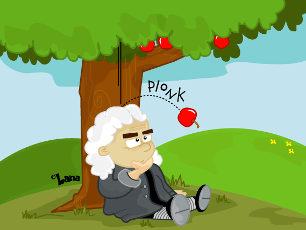
\includegraphics[width=0.3\textwidth]
    {newton_applepng.png}
\end{SCfigure}

Галилея также судили, приказывали признать, что все это ересь и отказаться от своих слов. Появление нового научного метода – эксперимент (индуктивный метод- от частного к общему). «Любая революция нуждается в хороших пропагандистах, и люди провозглашали, что «новые» научные ценности и практики удивительны, в то же время указывая на то, что древние и традиционные были полны ошибок» -побуждение людей к действиям, направленным на прогресс, на совершенствование мира. Самые важные достижения в науке XVII века благодаря Ньютону – физику, алхимику. Главной его работой стала новая методология. Также серьезная работа-«Начала математики» - 1687 год. Тут Исаак Ньютон собрал множество своих выводов об устройстве мира. Великие географические открытия сыграли важную роль в научной революции. Войны и болезни также можно отнести к факторам, которые двигают науку вперед (изобретение новых лекарств, прорывы в биологии и анатомии, разработка новых орудий/оружий).



В общем и целом:

\begin{enumerate} % nested
    \item что дала научная революция?
    \begin{enumerate}
        \item  открыла путь к новым знаниям
        \begin{enumerate}
            \item перед обществом встал совсем иной мир, 
   			\item мир, каким общество не привыкло его видеть
            \begin{enumerate}
                \item Картину мира после научной революции можно считать первой (объективной) картиной мира.
            \end{enumerate}
        \end{enumerate}
        \item  открыла путь к новым методам изучения
    \end{enumerate}
    
\end{enumerate}
 


\section{Размышление о гильотине}

\begin{figure}[h]
\centering

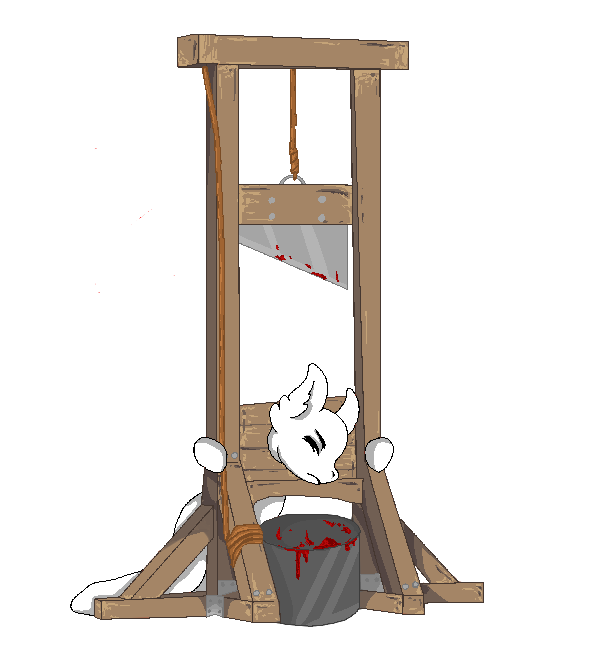
\includegraphics[angle=35,origin=c, width=0.3\linewidth]{guillotine.png}
%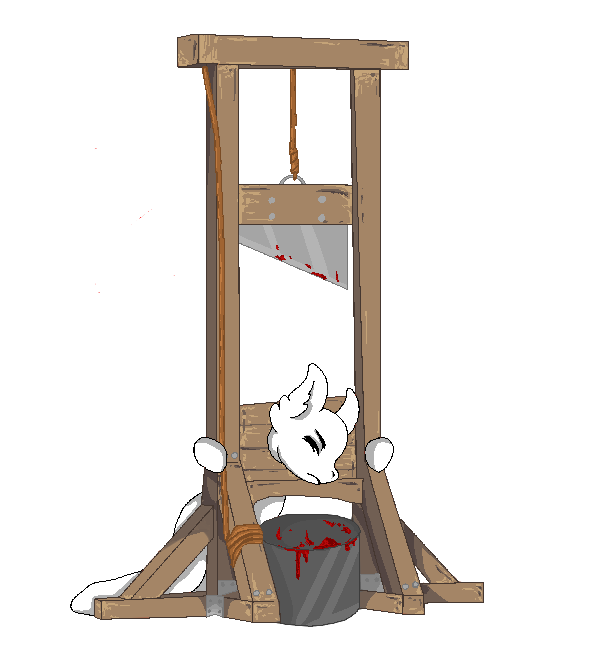
\includegraphics[width=0.4\linewidth]{guillotine.png}
\caption{Рисуночек с гильотиной}
\label{fig:mpr}
\end{figure}

В Алжире в 1914 году был приговорен к смертной казни один убийца, который убил всю семью с детьми и обокрал их. Казалось бы, все считали, что для него даже смертная казнь будет слишком мягка. Но после казни, пришедшие домой люди были в шоке от случившегося. Никто не решался даже заговорить о том, что произошло в то утро. И когда у обычных граждан на лицо после увиденного только ужас, возникает вопрос, а действительно ли данное свершение правосудия служит для поддержания порядка в стране. Это, напротив,
точно так же плохо, как и само убийство, совершенное преступником. Ведь эту ужасную смертную казнь представляют как  \footnote{First document. This is a simple example} необходимость. С одной стороны, узаконивается убийство, но с другой общество его не принимает и считает это дело мерзким и неправильным.

Произоше случай в Польше- публично казнили заложников. И мы видим, что невиновность лишается своих прав, а люди прикрывают казнь, законность которой невозмоможно подтвердить. Вместо того, чтобы заявлять, что смертная казнь необходима и затем уже не говорить о ней, стоило бы рассказать о том, что она представляет собой в действительности. Поэтому ответственность должна быть определенасамим обществом на основе разумной и эффективной шкалы, а не приравнивать все к смертной казни.

Все знают, что весомым аргументом смертной казни является назидательность наказания.Людей публично казнят не только для того, чтобы вершить правосудие над преступниками, но и для того, чтобы устрашающим примером запугать тех, кто пошел бы по их стопам. Общество потрясает людей для того, чтобы потенциальные убийцы увидели в этом свое будущее и одумались.
Но есть факты, доказывающие обратное: 

\begin{enumerate} % ordered
    \item Что общество само не верит в силу примера, о которой оно говорит;
    \item Что не доказано, будто смертная казнь уже заставила остановиться хотя бы одного убийцу, решившегося на такое преступление, и вместе с тем очевидно, что она не вызвала у тысяч преступников никакой реакции кроме восхищения;
    \item Что в других отношениях она является отвратительным примером, последствия которого непредсказуемы.
\end{enumerate}


 Не даром убеждение Кёстлера состоит в том, что “смертная казнь позорит наше общество, и ее сторонники не могут ее оправдать с точки зрения разума”.Для того, чтобы казнь имела показательный характер нужно либо запугать народ окончательно и представить все в полных красках, чтобы все видели этот ужас, либо прекратить говорить, что данное мероприятие имеет назидательный позыв. Ведь смертная казнь служит лишь для того, чтобы периодически информировать граждан о том, что они умрут, если им случится кого-то убить; такое же будущее можно смело обещать и тем, кто не убивает. Но как в момент совершения преступления будущий преступник может думать о наказании, которое представляют все более и более туманно?! Вместо того, чтобы в размытой форме говорить и страшном наказании, люди должны увидеть, насколько это страшно и противно. Для того, чтобы сделать это, надо дать людям почитать заключение врачей о том, что тело еще несколько минут живет после того, как вам отрубят голову и дергается и только потом умирает, а рот может кривиться в ужасной гримасе. Ведь только после этого можно говорить о том, что данная казнь является примерной для общества.
 

Я согласна с позицией автора, который считает смертную казнь болезнью обществ: она мерзкая и не приносит позитивных эмоций. Данный текст показывает, что при таком раскладе и при таких обстоятельствах, когда все более размыто готовят о “свершении правосудия” никакой потенциальный преступник не будет знать, как это ужасно оказаться на плахе, и чем это является на самом деле. Ведь даже врачи находятся в шоке от анализа тела после казни, ( а ведь они видели не мало) потому что тело еще живет и подает хаотичные непонятные признаки жизни без головы. Но я не согласная с его позицией о том, что человек по своей природе это не общественное животное, ведь все личные качества человека и его характер появляются только от взаимодействия человека с обществом. Только так он может раскрыть свои умственные и социальные качества, а также сформировать свое представление о мире и тем более отношение к миру. Ведь все социальные качества и влияние общества на человека влияют на то, кем станет человек, и будет ли он преступником или нет.     

\begin{wrapfigure}{r}{0.5\textwidth}
  \vspace{-20pt}
  \begin{center}
    
\includegraphics[width=0.48\textwidth]{mickey_mouse.jpeg}
  \end{center}
  \vspace{-20pt}
  \caption{Микки} 
  \vspace{-10pt}
\end{wrapfigure}

Автор\cite{cederstrom2012dead} данного текста во всех красках показывает, почему смертная казнь несет обществу только вред. В наше время нет публичной смертной казни, она производится только если в тюрьмах и со специальными людьми. В настоящее все преступники, которые осознанно шли на нарушение закона, знали, что будет в тюрьме и к чему это все приведет\cite{holt1972some}. То, что происходит в местах для заключенных не является секретом и любой взрослый человек знает, что его ждет в случае нарушения закона. Также каждый случай рассматривают\footnote{На этой странице цитаты} отдельно\cite{lassauce2011deadwood} и каждому злодею свои приговор и свой вид ответственности, так как есть четкие границ\cite{bronfen2017over}, прописанные в    конституции РФ. В настоящее время не уравниваются два совершенно по-разному весящих преступления, например, как убийство и грабеж. Каждому свое наказание\cite{normey2007control}.
\section{Как публично сквернословить?}

В одной из своих “картонок” Умберто Эко осветил не столь явную проблему общества, но очень важную. Этой проблемой является сквернословие людей. Все больше людей в своей повседневной речи употребляют нецензурные слова. Сейчас очень редко можно встретить человека, не употребляющего в своей речи неподобающие для общества слова. В нашей стране сквернословят люди, относящиеся практически ко все социальным слоям. Мы нередко можем услышать матерные слова по телевизору, радио и даже в детском саду от детей! Большинство людей относятся к ненормативной лексике нормально, считая ее лишь средством выражения эмоций. Автор в своей “картонке” пишет как раз о том, что сам отстаивал мнение о том, что можно использовать некоторые слова как высшую степень негодования происходящим. А вот использовать матерщину слишком часто очень некрасиво для человека вне зависимости от его статуса и положения в обществе. Тем более, что чрезмерное употребление нецензурных слов грозит плохими последствиями, как и говорящему, так и окружающим его людям. Если разобраться с точки зрения истории, что значит “мат”. Ученые выяснили, что матерная брань- обращение к языческим духам. Многие слова, которые человек употребляет по несколько раз за день являются именами тех самых духов и богов, а другие- страшными проклятиями. Наши предки осознавали вред данных слов, и поэтому им нельзя их было употреблять чаще, чем 10 раз в год, а тем более в общественных местах. Не все люди понимают количество вреда, которое приносят бранные слова. Употребление подобных слов при детях, думая, что они их не запомнят, опрометчиво.  Ведь именно эти слова дети и будут запоминать, потому что родители употребляют их на эмоциях, а именно это и важно для “маленьких” людей. Такое воспитание влияет на дальнейшую судьбу и поведение ребенка, ведь малыши копирую своих родителей и подражают им. 


\begin{wrapfigure}{l}{0.5\textwidth}
  \vspace{-20pt}
  \begin{center}
    
\includegraphics[width=0.48\textwidth]{mouse.jpeg}
  \end{center}
  \vspace{-20pt}
  \caption{Мышь} 
  \vspace{-10pt}
\end{wrapfigure}

Также огромный вред нецензурные слова оказывают и на самого говорящего. Матерные слова имеют большую зависимость, даже если она не заметна. Но некоторые ученые сравнивают ее с наркологической и алкогольной. Такие слова через время будут заменять большинство слов из лексикона человека. Одно матерное слово займет место десяти других, и со временем культурные и изящные слова человек может забыть, и в эмоциональной ситуации только вредные слова и будут вылетать. Именно ухудшение словарного запаса и происходит от использования в речи неподобающих слов. Употребление ненормативной лексики в тюрьме запрещено, потому что матерные слова содержат понятные всем оскорбления, которые заключенные могут трактовать вполне буквально и “отплатить” говорящему сполна. В православии сквернословие – это грех, который неугоден Богу. К тому же многие матерные слова являются настоящим и страшным оскорблением для Божьей Матери. С каждым таким словом мы отдаляемся от Бога и у нас все меньше шансов на искупление и вступление в рай после смерти. 

Проанализировав с разных сторон пользу и вред ненормативных слов, можно понять, что пользы в них никакой нет, а только лишь огромный вред. Каждый человек относится к смыслу употребляемых сов индивидуально, но не все анализируют происходящее с ними. Умберто Эко указал на искусство оскорбления, воспетое Борхесом, которое уже утрачено. Автор показал хорошую возможность исправлять тот вред, что нанесли нецензурные слова человеку - совершенствоваться в искусстве парафазы. Употребленные выражения утонченные и изящные, но в то же время имеют жесткий смысл и конкретный мотив. Эти варианты ничуть не уступают в крепости нецензурным словам. Данное искусство несет пользу и позволяет обогатить свой словарный запас, при этом аккуратно “подкалывая” людей колкими фразами из культурных слове\footnote{Поэт выделяет беспомощность людей перед барином в стихотворении “В
деревне”, где девушку, которая долгое время воспитывалась в господском
доме как подруга маленькой барышни, но по стечению обстоятельств новый
барин отправил девушку в крестьянскую избу, предварительно выдав замуж.}. 


\chapter{Таблицы}
\section{Задача }
\textbf{Формулировка:   }
По данным ниже приведенных таблиц найдите количество детей, у которых

\begin{itemize}[noitemsep] %unordered
    \item Их статус по наличию родинок совпадет с бабушкой/дедушкой.
    \item На момент их рождения этой/этому бабушке/дедушке было меньше 55 лет.
\end{itemize}


\begin{flushleft}
\begin{tabular}{ | c | c| c |c|c| }
\hline
\rowcolor[gray]{.6} \textbf{ID} & \textbf{Имя} & \textbf{Дата рождения} & \textbf{Пол  человека} &\textbf{Есть ли родинки }\\ \hline
\rowcolor[gray]{.9} 11 & Иван & 1970.11.07 & М & Да \\
\rowcolor[gray]{.9} 15 & Валерия & 1941.05.19 & Ж & Да \\
\rowcolor[gray]{.9} 34 & Ольга & 1966.02.10 & Ж & Нет \\
\rowcolor[gray]{.9} 42 & Олег & 200.04.01 & М & Нет \\
\rowcolor[gray]{.9} 51 & Дмитрий & 1963.10.25 & М & Да \\
\rowcolor[gray]{.9} 13 & Кирилл & 1997.10.25 & М & Нет \\
\rowcolor[gray]{.9} 18 & Даниил &1944.09.17 & М & Нет \\
\rowcolor[gray]{.9} 25 & Максим &1964.12.15 & М & Да \\
\rowcolor[gray]{.9} 26 & Василиса & 1945.03.22 & Ж & Нет \\
\hline
\end{tabular}\\
\end{flushleft}





Ну и сама таблица с родителями и детьми \footnote{First document. This is a simple example}: 
\begin{tabular}{%
|>{\color{blue}\columncolor[gray]{.9}}c|
>{\color[gray]{.9}\columncolor{blue}}c|}
\hline
 \textbf{ID родителя} & \textbf{ID ребенка}  \\ \hline
 11 & 17 \\
51 & 42 \\
 51 & 13 \\
 26 & 51 \\
 26 & 11 \\
 26 & 34 \\
25 & 14 \\
34 & 14 \\
\hline
\end{tabular}
\clearpage




\chapter{Формулы}
\section{ Формула 1}


\[\binom{n}{a_{1} , \cdots, a_{k}, a_{k+1}} = \binom{n}{j}  \binom{j}{a_{1} , \cdots, a_{k}} = \frac{n!}{j!(n-j)!} \cdot \frac{j!}{a_{1}!a_{2}! \cdots a_{k}! } = \frac{n!}{a_{1}!a_{2}! \cdots a_{k}! (n-j)! }\]

\section{ Формула 2}

\[ y = \ln {\sqrt[5]{\frac{1-x}{1+x}}} = \ln {\left( {{1-x}\over {1+x}} \right)^{\frac{1}{5}}} = \frac{1}{5} \ln {\left( {{1-x}\over {1+x}} \right)}
= \frac{1}{5} \left( {\ln{\left( {1-x } \right)}  - \ln{\left( {1+x } \right)}} \right)\]

\section{ Формула 3}

\[\frac{\frac{\left({\cos {x} - \sin{x} }\right) \cdot  
\left({x^{3} + {3}{x}+1} \right) - x \left({x^{2} + 1} \right) \cos{x}}
{\sqrt[3]{\left({{x^{3} + {3}{x}+1}}\right) ^{2}}}}{\sqrt[3]{\left({{x^{3} + {3}{x}+1}}\right) ^{2}}} = \] 

\[ = {\frac{\left({\cos {x} - \sin{x} }\right) \cdot  
\left({x^{3} + {3}{x}+1} \right) - x \left({x^{2} + 1} \right) \cos{x}}
{\sqrt[3]{\left({{x^{3} + {3}{x}+1}}\right) ^{4}}}} \]

\section{ Формула 4}

\[ y' = {\left({\arctan^{3} {2x} \cdot \cos{8x} }\right)'} = {\left({\arctan^{3} {2x}}\right)' \cos{8{x}^{5}}} + {\arctan^{3} {2x}}{\left({\cos{8{x}^{5}}}\right)'} = \]

\[ = {3\arctan^{2}{2x} \cdot \left({\arctan {2x}}\right)' \cos{8{x}^{5}}} - {{\arctan^{3} {2x}} \cdot \sin{8{x}^{5}} \left({{8{x}^{5}}}\right)'} \]





\bibliographystyle{plain}
\bibliography{bib.bib}



\end{document}
